

\chapter{Algorithmic Complexity and Complexity Analysis}

The efficiency of an algorithm can be measured by estimating how long the algorithm will take to complete for some set of data, and by
estimating how much memory the algorithm will require to perform that execution. The context of your computing environment tells you which
measure is most important. If you have limited memory you will require an algorithm that uses minimal memory. If you need an answer very
quickly, you will require an algorithm with fast execution time.   The estimate of the efficiency of an algorithm is known as the algorithm's \textbf{complexity}.



\subsection{Determining Complexity}

We often need to know the complexity of a particular algorithm.     We could attempt to experimentally determine the running time of an algorithm,  or we could analyse the algorithm theoretically.   


\subsubsection{Experimental Analysis}

In order to experimentally analyse an algorithm, we first must implement the algorithm.  This seems like an obvious step, but if we're trying to choose between three competing algorithms,  the experimental analysis means that all three algorithms must be implemented.    Sometimes that is trivial,  sometimes it is not.

After the algorithm is implemented,  we must \textbf{instrument} the algorithm to enable us to measure the running time.   Usually that means using  some kind of timer or clock.       Below is a sample testing function that uses two fictional functions,  Sort() and Time().  Sort() is the function being analysed.  Time() is the function used to capture the time in seconds since midnight.   

\begin{lstlisting}
float testSort( List * the List)
{
    float seconds = 0.0;
    float time1, time2;
    time1 = Time();
    Sort(theList);
    time2 = Time();
    seconds = time2-time1
    return seconds;
}
\end{lstlisting}

The testSort function would be run with a variety of lists using different sizes and compositions of data.   The results would be analysed statistically to determine  the best, worst, and average running time of the algorithm, and what data characteristics affect those times.

While this process sounds straightforward,  there are several  possible issues that can make consistent analysis difficult.  For example:

\begin{itemize}
\item What language should be used for testing running time of the algorithm?   Some languages might offer facilities that significantly slow down, or speed up some operations.
\item What compiler should be used?  Some languages (like C) have different compilers available.   Each compiler is slightly different and will result in different running times.
\item What hardware environment should be used?  Will the results from running on a new  hardware system be the same as running on a system that is several years old?
\item What software should be used?  Will the results from running on a Windows operating system be the same as the results from running on a linux system?   
\item How do we select the data to be input?   If two different testers make test data, will the results be the same?

\end{itemize}

Clearly, it is much more difficult to get consistent measurements of running time experimentally than it seems.    Most often we content ourselves with a theoretical analysis of the algorithm.  This theoretical analysis does not have to be formal (in the sense that it requires a full blown proof).  


\subsubsection{Theoretical Analysis}
Theoretical analysis of algorithms has the advantage that the running time of the algorithm can be evaluated without having to implement the algorithm,  while taking into account all possible inputs, independently of hardware and software.

We perform a theoretical analysis by counting the primitive operations in an algorithm.  Primitive operations include assignments, comparisons and arithmetic operations.     This counting exercise must take into consideration the effect of the size of the input values.  The size of the input usually  impacts things like the number of iterations of a loop or the length of an array.

Consider the code(shown below)  for finding the maximum value in a list of integers.    The code assumes that the List ADT has functions for getting the value of an element at a specific place and for finding the length of the list.   We'll assume, for the purposes of this analysis,  the the running time for all the list operations used in the example is O(1) or constant time.

\begin{lstlisting}
int findMax(List theList)
{
    int currentMax = getFirstElement(theList);
    int i;
    for(i = 1; i<length(theList); i++)
    {
    	tempElement = getElement(theList, i);
        if (tempElement > currentMax)
            currentMax = tempElement;
    }
    return currentMax;
}
\end{lstlisting}

A count of the primitive operations in this code (where n = length of the list) yields the following:

\begin{table}[H]
\begin{tabular}{l || l}
    int currentMax = getFirstElement(theList); & 2 (assignment and list function call)\\ \hline
    int i = 0; & 1 (assignment)\\ \hline
    for(i = 1; i<length(theList); i++) & 2(n-1)+1 (1 assignment plus n-1 comparions and n-1 increments of i)\\ \hline

    	tempElement = getElement(theList, i);  &  2(n-1) (2 operations done n-1 times)\\ \hline
        if (tempElement > currentMax) & n-1 (1 comparison done n-1 times)\\ \hline
            currentMax = tempElement; & n-1 (1 comparison done n-1 times)\\ \hline

   return currentMax; & 1 \\ \hline
\end{tabular}
\end{table}

This algorithm only runs through the entire list if the largest value in the list is in the last position of the list.  That is called the \textbf{worst case}.  In the worst case, the algorithm executes 5 + 6(n-1), or 6n -1  primitive statements (with the assumption that the list functions are the equivalent of a primitive statement).     

Lets suppose that there was one specific primitive operation that took longer than the others, and one that was faster.   Without doing an analysis to determine exactly the speed of each primitive operation,  we can say that the fastest execution speed would occur if all the primitive operations were the fastest operation.   We can also say that the slowest execution speed for this algorithm would occur if all the primitive operations were the slowest operation.    So the execution speed of the function, is bounded by the fastest/slowest speeds of the primitive operations.

For the purposes of estimating complexity of algorithms, we assume that primitive operations take \textbf{constant time} and don't worry too much about exactly how much time that is.    Using that knowledge we can say that the algorithm above takes   6n -1 constant time units based on the worst case analysis.   

    This means that the execution time of the algorithm depends on the length of the  list (n).   We say that such an algorithm is \textbf{Order N} or \textbf{O(N)}.

\subsection{Big O notation}

 Time
complexity is often expressed in Big O notation.
The big O is read as
\textbf{on the order of},which means that the most significant factor in the
time complexity analysis is shown.   The \textbf{N}  represents the data input into the algorithm.  

So if we say that an algorithm is
O(N) (read that as order-N),we mean that the upper bound on execution
is controlled linearly by the number of input data.  We do NOT mean that the
algorithm will take exactly N time to complete.  


Big O notation signifies an \textbf{upper bound } on the complexity/computational
time for an algorithm.  The term upper bound means that the algorithm might run faster, but won't run
slower.

Big O notation usually describes worst case, but sometimes it is given
for average and best case too when that can be clearly defined. The
complexity measure describes a relationship between the size of the
input data (how much data goes in) and the time the algorithm will take
to run.  Typical Big O  values are O(1) or constant time, O(N) or proportional to data size, and O(n\textsuperscript{2}), which means that execution will take approximately as long as the square of the size of data.  We'll learn about each of these types of algorithms as well as others during the course of this class.

\subsection{Estimating Complexity}

Imagine that you are estimating the number of days required for an
automobile trip across Canada. Your estimation would likely include the
distances between major cities, but you would be unlikely to factor in
the short side trips into small centers for gasoline, or trips into
museums or tourist sites. The most significant distances are the ones
between the cities so those become the basis for your overall estimate
of trip time.

When you are estimating time complexity of an algorithm, you also ignore the
"side trips", or the parts of the program that don't contribute much to the overall execution time.
When calculating computational complexity we ignore things like the programming language used, the characteristics of the compiler, and the
speed of the computer that will be used to run the program. The time
complexity of the algorithm is based on the characteristics of the
algorithm alone.

Big-O lets you compare the complexity of algorithms that do similar
operations. It provides a way to estimate the number of operations
required to complete an algorithm. We assume that the operation that
is executed the most is the one that should be counted, and that we can
ignore other operations because the time added won't significantly impact
the overall time. We also ignore anything that takes a constant amount
of time.


Complexity analysis is used most often in situations where the algorithm
is processing data and the set of data can vary in size.  For example,
suppose you have written a stack library and you want to know how its algorithms
compare to those in other libraries.  One way to compare is to analyze how much
processing effort is required for your stack's algorithms to work with an
arbitrary size of data (N). If the stack must go through the entire set
of data once, we say it is O(N).  If the stack library must go through
the set of data in a nested loop, we say it is O(N\textsuperscript{2}).

For this course we will focus on six categories of computational
complexity- O(1), O(logN), O(N), O(NlogN), O(n\textsuperscript{2}), O(2\textsuperscript{N}).  At the
conclusion of the course you will know the characteristics in code that
are associated with each category of complexity and you should be able
to estimate the complexity for several different types of  algorithms from those efficiency classes.


\subsection{Complexity in the real world}

This section presents an easy to understand, real world,  example of algorithm
complexity using a printed phone book.  In this example \textit{N} represents
the number of entries in the phone book.  The example is copied verbatim from:


\url{http://stackoverflow.com/questions/2307283/what-does-olog-n-mean-exactly}

\begin{displayquote}

{We will assume our phone book has \emph{{businesses}}(the \textit{Yellow
Pages}) which have unique names and \emph{{people}}(the \textit{White Pages})
which may not have unique names. A phone number is assigned to at most
one person or business. We will also assume that it takes constant time
to flip to a specific page.}

{Here are the running times of some operations we might perform on the
phone book, from best to worst:}

\begin{itemize}
\item
  \textbf{{O(1)(worst case):}}{Given the page that a business's
  name is on and the business name, find the phone number.}
\item
  \textbf{{O(1)(average case):}}{Given the page that a person's
  name is on and their name, find the phone number.}
\item
  \textbf{{O(log n):}}{Given a person's name, find the phone
  number by picking a random point about halfway through the part of the
  book you haven't searched yet, then checking to see whether the
  person's name is at that point. Then repeat the process about halfway
  through the part of the book where the person's name lies. (This is a
  binary search for a person's name.)}
\item
  \textbf{{O(n):}}{Find all people whose phone numbers contain the
  digit ``5''.}
\item
  \textbf{{O(n):}}{Given a phone number, find the person or
  business with that number.}
\item
  \textbf{{O(nlog n):}}{There was a mix-up at the printer's
  office, and our phone book had all its pages inserted in a random
  order. Fix the ordering so that it's correct by looking at the first
  name on each page and then putting that page in the appropriate spot
  in a new, empty phone book.}
\end{itemize}

{For the below examples, we're now at the printer's office. Phone books
are waiting to be mailed to each resident or business, and there's a
sticker on each phone book identifying where it should be mailed to.
Every person or business gets one phone book.}

\begin{itemize}

	\item \textbf{{O(n log n):}}{We want to personalize the phone book, so
we're going to find each person or business's name in their designated
copy, then circle their name in the book and write a short thank-you
note for their patronage.}

	\item \textbf{{O(n}\textsuperscript{{2}}{):}}{A mistake occurred at the
office, and every entry in each of the phone books has an extra ``0'' at
the end of the phone number. Take some white-out and remove each zero.}

	\item \textbf{{O(n!):}}{{}}{We're ready to load the phonebooks onto
the shipping dock. Unfortunately, the robot that was supposed to load
the books has gone haywire: it's putting the books onto the truck in a
random order! Even worse, it loads all the books onto the truck, then
checks to see if they're in the right order, and if not, it unloads them
and starts over. (This is the
dreaded bogo sort} \url{http://en.wikipedia.org/wiki/Bogosort}

	\item \textbf{{O(n}\textsuperscript{{n}}{):}}{{}}{You fix the robot so
that it's loading things correctly. The next day, one of your co-workers
plays a prank on you and wires the loading dock robot to the automated
printing systems. Every time the robot goes to load an original book,
the factory printer makes a duplicate run of all the phonebooks!
Fortunately, the robot's bug-detection systems are sophisticated enough
that the robot doesn't try printing even more copies when it encounters
a duplicate book for loading, but it still has to load every original
and duplicate book that's been printed.\\
}

\end{itemize}
\end{displayquote}



\section {Analysis of Algorithms using Big O}

When arriving at the Big O complexity for an algorithm, we count the number of primitive operations.  We then select the term with the highest order in the resulting sum to use as the complexity.    The lower order terms, and any constant terms, will not add to the overall execution time since the higher order term dictates a longer time than required by lower terms.

The following guidelines apply:

\begin{itemize}
\item If the sum is a polynomial where the highest degree is $d$ then the algorithm is $O(N^d)$
\begin{itemize}
\item Suppose the sum of the primitive operations is $6n^2 + 5n + 10$
\item We first drop the lowest order terms to arrive at $6n^2$
\item We then drop any constants to arrive at $n^2$
\item The algorithm would be $O(N^2)$
\end{itemize}
\item Use the smallest possible order to describe the complexity
\begin{itemize}
\item If the sum of the primitive operations is $2n$  say that the algorithm is $O(N)$ rather than saying it is $O(N^2)$
\item Even though $O(N^2)$ is technically correct, because the algorithm will not run slower than that, it is not as informative, since the algorithm will also run an order faster.
\end{itemize}
\item Use the simplest expression of the order
\begin{itemize}
\item If the sum of the primitive operations is $3n+5$  say that the order of the algorithm is $O(N)$ rather than $O(3N)$
\end{itemize}

\end{itemize}

The computational complexity of an algorithm is not an exact measurement of the running time of an algorithm.   Rather it is an estimate of the time that allows us to classify the algorithm into one of several \textbf{complexity classes}.   Complexity classes are divided into three categories,  constant, polynomial and exponential.    We'll explore several complexity classes in the next few sections.

You begin an analysis of an algorithm by counting.   There is no real need to count the executions for every step of an algorithm, since we know that we are only interested in the higher order execution times.   In particular,  focus the analysis on section of the algorithm that go through the input data item by item.  

\begin {itemize}
\item Count the number of arithmetic operations performed
\item Count the number of comparisons made
\item Count the number of variable assignments
\item Count the number of array elements accessed 
\item Count the number of times each loop executes
\end{itemize}



\textbf{Example:}

Below is an example program that can be used to illustrate how to
calculate complexity. The complexity of each line of the program is
explained in the table following the source code listing. For this example, assume that N represents the
number of data items the algorithm must process.

\begin{center}
\begin{lstlisting}
int n=100;
int w = 0;
for(int i=1; i<n; i++)
{
	for(int k=1; k<n+n; k++)
	{
		w = w+1;
	}
}
\end{lstlisting}

\begin{table}[h]
\caption{Big O analysis of simple C program}
\begin{tabular}{l || l}
int n=100; int w=0;& These two assignments happen once each so they are O(1)\\ \hline
for (int i=1; i\textless n; i++) & This loop will execute n times so the loop is O(N)\\\hline
for (int k=1; k\textless n+n; k++) & This loop will execute 2n times.  That is still considered to be O(N)\\\hline
{  w=w+1;} & \specialcell[]{Assignment happens once for each inner loop iteration. (N outer loops X 2N inner loops) \\The assignment occurs N*2N times, which is O(N\textsuperscript{2})}\\\hline\hline
\end{tabular}

\end{table}
\end{center}

\subsection{Analyzing recursive functions}

A recursive algorithm can be analysed for complexity using the same process of inspection.   The only difference is that the repetition in a recursive algorithm happens during the recursion,  so counting the number of primitive operations requires an understanding of how many times the recursion will be invoked.

\begin{lstlisting}
int power (int num, int power) {
    if(power==0)
    {
        return 1;
    }
    else
    {
        return num * power(num, power-1);
    }
}
\end{lstlisting}

The program  shown above uses recursion to calculate the result of applying an exponent (power) to a number (num).   
An analysis of the algorithm is shown in the table below.

\begin{tabular}{l|l}
 if(power==0) & 1 (one comparison)\\ \hline
       return 1; &  1 (one return)\\ \hline
       return num * power(num, power-1); & 1 (return) + 1(multiplication) + (power-1)* the running time \\\hline
\end{tabular}

The calculations in the algorithm run in constant time ( a return statement, a comparison and a multiplication)  but those calculations must happen once for every time through the recursion.   The recursion happens (power-1) times after the first pass through the algorithm.   So the complexity if the algorithm is O(N)  where N = power.

\subsection{O(1) and O(N)}

\subsubsection{Constant Time- O(1)}

If an algorithm  runs in constant time the complexity of the algorithm is independent from the size of the
input.  No matter how big the input is, the algorithm requires the same amount of time to execute.

An algorithm that looks up elements in an array is O(1) because it takes
the same amount of time to access any element regardless of where the
element is in the array (assuming you know the index of the element).
An algorithm that returns a value, such as the date, time, or
characteristics of the operating system is O(1). An algorithm that
always returns the same value (maybe a zero) regardless of the data
involved is also O(1).



\begin{itemize}
\item
  A program to determine characteristics of numbers (odd/even/divisible
  by 3, power of 2, etc)
\item
  A program that looks something up in a constant sized array or hash
  table,
\end{itemize}



\subsubsection{O(N)}

The performance of an O(N) algorithm  is directly
proportional to the size of the input data.

An algorithm that runs in O(N) can perform all of its necessary
processing by handling each element of data only once.  When the data
grows in size, the length of time taken by the algorithm increases by a
similar proportion.  Twice as much data will take twice as long to execute.  Reducing the data by 1/3 will reduce the time required by 1/3.
Some examples of O(N) algorithms include:

\begin{itemize}
\item
  \textbf{} Looking through an unsorted array or linked list is an O(N)
  operation.
\item
  Copying a set of data  from one memory location to another is O(N).  \textit{Realloc} peforms a copy from one memory location to another if necessary when it is called.
\item
  Creating a sum from a list of numbers is an O(N) operation.
\end{itemize}



\subsection{O(logN)}

O(logN)suggests that the algorithm will take
log\textsubscript{2} N time to complete, where N is the size of the
input. This means that the time required increases linearly while the
size of the input increases exponentially.

Most often, O(logN) refers to log (base 2) of N. You can think of this
as the number of times you can divide the set of things into 2 (the
base) before you reach sets of one.An algorithm that os )(logN) often
divides the set of data as part of its operation.   Operations on binary trees are usually O(logN).

Searching a binary tree (a balanced one) is one example of an algorithm
that takes O(logN).If the binary tree has 8 elements in it, thenyou can find any element in the tree in 3 or fewer steps. This
makes sense because the maximum depth of a 8 element balanced tree will
be 3.

A binary search of an array is also an O(logN) operation.  Suppose we were searching the array shown below for the value 89.  A binary search begins by examining the middle element in the sorted list.

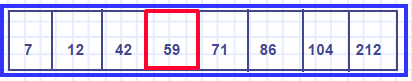
\includegraphics{pictures/binarySearch1.png}

Since our target value (89) is more than the value of the middle element of the list (59) we can immediately disregard the first half of the list  for the rest of the search.   We then search for the target value in the second half of the list by starting at the mid point of the second half.

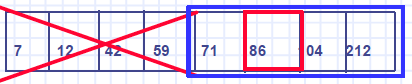
\includegraphics{pictures/binarySearch2.png}


The target value is larger than the midpoint value, so we once again ignore the first half of the list and repeat the search on the last half of the list.

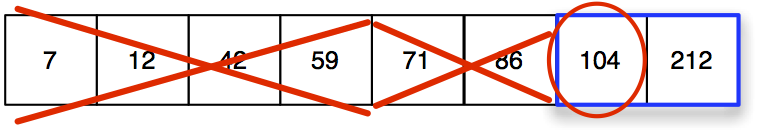
\includegraphics{pictures/binarySearch3.png}

This time the  midpoint value is larger than the target value, which tells us that our target value is not in the array of values.


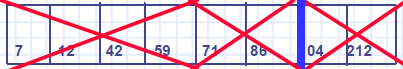
\includegraphics{pictures/binarySearch4.png}

The search concluded with 3 comparisons.   Log(8)  is 3.  A binary search is an O(logN) algorithm.


Logarithmic algorithms often use a divide and conquer strategy to manipulate the data.   Often there is some kind of selection step in a logarithmic algorithm that permits the algorithm to ignore some part of the data, thus speeding up the algorithm.


More information about O(log N) can be found here:
\url{http://stackoverflow.com/questions/2307283/what-does-olog-n-mean-exactly}


Some common algorithms that are O(logN) include:
\begin{itemize}

\item binary search of a sorted array is O(logN)
\item many algorithms using tree data structures are O(logN)
\item  computing the answer to x\textsuperscript{N{ }}is O(logN)
\end{itemize}


\subsection{O(NlogN)}

An O(NlogN) algorithm is one that divides the input data
up in a similar fashion to an O(logN) algorithm but then performs an O(N)
operation on each of the halves of the data.   An O(NlogN) algorithm does not entirely skip the processing for any of the data elements.

Good sorting algorithms are O(NlogN). A good description of O(NlogN) can
be found here: \url{http://www.crsr.net/Notes/BigO.html}. This article
is also a great review of Big O notation in general- it is worth reading the whole
thing.

A mergesort is a great example of an algorithm that os O(NlogN).   Recall that a merge sort has two phases:

\begin{itemize}
\item Phase 1
\begin{itemize}
\item Divide the list of N elements into two lists of N/2 elements
\item Divide those two lists in half
\item repeat the division until each least is length 1
\item This phase has log N steps
\end{itemize}
\item Phase 2
\begin{itemize}
\item Starting from the lists of length one, create a sorted list from each pair of lists
\item continue merging paired lists, doubling the size of the sorted list with each merge
\item This phase has log N steps or passes.   
\item For each of the log N passes,  every element in the input data is compared or copied.   
\item Each pass is O(N) and there are log N passes, giving O(NlogN) for the sort
\end{itemize}
\end{itemize}





\subsection{O(n\textsuperscript{2})}

An O(n\textsuperscript{2}) algorithm (or an
O(n\textsuperscript{k})) is one that runs in polynomial time with
respect to the size of the input.This means that as the input size
increases, the time required by the algorithm increases by some
polynomial factor (squared, cubed, etc).

O(n\textsuperscript{2}) algorithms take more time for
large input than logarithmic and linear algorithms, but are still
considered to be reasonably good algorithms for some types of problems as long as the value of k is small(typically 2 or 3)
Any nested loop that goes through the input data in both loops is an
O(n\textsuperscript{2}) algorithm.
An O(n\textsuperscript{2})
algorithm is one that performs an operation on every data element while looping through the set of data elements.  

For example,  suppose we implemented a simple algorithm for finding duplicates in an array.     

\begin{lstlisting}
void printDuplicates(int * theArray,  int length)
{
    int j, k;
    for (j = 0; j < length; j++)
    {
      for(k=0; k<length; k++)
      {
          if( k!=j && theArray[k] == theArray[j])
              printf("Found duplicates at positions %d and %d", j, k);
      }
}
\end{lstlisting}

This algorithm selects an element in the array and then compares it to every other element in the array to check for duplicates.  It performs this step once for every element in the array.     The complexity of this algorithm is $O(N^2)$

\begin{itemize}

\item Bubble Sort, Insertion Sort and Selection Sort are O(n\textsuperscript{2}) algorithms.\\
\item  Some text processing algorithms are intuitively  O(n\textsuperscript{2}) such as checking a list for duplicate words.
\end{itemize}



\subsection {O(2\textsuperscript{n})}

An algorithm that is O(2\textsuperscript{n}) will double in
complexity each time an additional data element is added. Such an
algorithm is said to have exponential complexity and is usually an
algorithm that is unlikely to complete in a reasonable time for most
sizes of input.

An exponential algorithm experiences rapid growth with
the size of the data set and is really only used in situations where the
size of data can be controlled or reduced prior to algorithm execution.

These types of algorithms are often the used to approximate solutions to
problems that are intractable- or problems that are not presently
solvable by computer. (more information on NP-Complete problems can be
found here \url{http://www.mathsisfun.com/sets/np-complete.html} or
\url{http://www.cs.berkeley.edu/\%7Edaw/teaching/cs170-s03/Notes/lecture21.pdf}

Examples:
\begin{itemize}

\item Many classic artificial intelligence problems have a solution that is
  exponential.
\item  The travelling salesman problem
\item the 8 queens problem
\item map colouring
\item  many graph algorithms (spanning tree, cycle detection).
\end{itemize}

\subsubsection {Understanding Exponential Growth}
 It is sometimes difficult to understand just how quickly the execution times increase when an algorithm has exponential complexity.  
 
 It is perhaps a little easier to consider the exponential increase of personal time.  Imagine that you were doing an activity that took you twice as long each time you did it.    The first time you did the task it would take  0.5 seconds.  The second time it would take 1 second.   The chart below shows the time involved for the first few attempts at the task.
 
\begin{tabular}{l|l}
attempt number & time to complete  in seconds\\ \hline
1 & 0.5 \\
2 & 1 \\
3 & 2 \\
4 & 4 \\
5 & 8 \\
6 & 16 \\
7 & 32 \\
8 & 64 \\
9 & 128 \\
10 & 256 \\
11 & 512 \\
12 & 1024\\ \hline
\end{tabular}

In 12 repetitions the task goes from something that can be done quickly to something that takes nearly 20 minutes.    If you imagine now that the task is something like sorting a list of numbers,  and that each attempt represents adding one more element to the list,  you can quickly see how dreadful the performance would be with even a short list of numbers.

The following story is often used to illustrate the power of exponential growth.

A peasant once did a great favour for a rich king.  The king asked how he could repay the peasant.   The peasant asked the king to place two pieces of grain on the first square of a chess board, and to double the amount of grain on each following square. The king, knowing that the chess board only has 64 squares, readily agrees.   However, the king does not understand exponents.

\begin{table}[H]
\caption{The King's payment for each square on the board}

\begin{tabular}{l|l}
Square(N)&Pieces of Grain\\\hline\hline
1&2\\
2&4\\
3&8\\
4&16\\
5&32\\
...&...\\
63 & 9 223 000 000 000 000 000\\
64 & 18 450 000 000 000 000 000\\
\end{tabular}
\end{table}

So just how much trouble will the king have repaying his debt?   Imagine that the king can grow 1 billion pieces of grain ever second.   It will take 585 years to grow enough grain for the 64th square on the chess board.   It would take over one thousand years to cover the entire chessboard using the peasant's algorithm.

\subsection{Reasonable vs Unreasonable algorithms}

Algorithms that are reasonable have polynomial complexity.   Such algorithms might run slowly, but they will eventually finish and return a value.
O(N), O(log N) and O(N\textsuperscript{k})  where k is some constant number are all examples of the complexity of reasonable algorithms.

Even a reasonable algorithm can be unusable if it is O(N\textsuperscript{k}) and k is a large number.

Unreasonable algorithms have exponential complexity.   Examples of exponential complexity are O(2\textsuperscript{n}), O(N!) and O(N\textsuperscript{N}).

\section {Additional Resources for Computational Complexity}

The internet has excellent resources for learning about computational
complexity. 

\begin{itemize}
\item \url{http://pages.cs.wisc.edu/~vernon/cs367/notes/3.COMPLEXITY.html}
\item  \url{http://stackoverflow.com/questions/107165/big-o-for-eight-year-olds}
\item  \url{http://www.perlmonks.org/?node_id=227909}
\item  \url{http://stackoverflow.com/questions/487258/plain-english-explanation-of-big-o}
\item  \url{http://www.crsr.net/Notes/BigO.html}
\item  \url{http://www.csd.uwo.ca/courses/CS1037a/notes/topic13_AnalysisOfAlgs.pdf}
\end{itemize}

\section{Extending Activities}

\begin{itemize}


\item  Assume you have a computer that can execute 1 billion instructions per second.  How long (in seconds/minutes/days/months/years) would that computer take to execute an algorithm of the complexity give for each of the number of data items shown.

\begin{tabular}{|l|c|c|c|}
	\hline
	Algorithm order & 10 000 data items & 1 million data items & 1 billion data items\\
	\hline\hline
	O(log N)& & &\\	\hline
	O(N)& & &\\	\hline
	O(N log N) & & &\\	\hline
	O(N\textsuperscript{2}& & &\\	\hline
	O(2\textsuperscript{N}& & &\\	\hline
		\hline
\end{tabular}

\item Create a table showing the count of the primitive operations for the algorithm for adding a node to the end of a singly linked list.  The algorithm is given in the Linked List materials for this course.   What is the big O complexity for that algorithm?

\item { Consider these three algorithms for determining whether anyone in a room of people has the same first name as a target person.
\begin{itemize}
\item The target person says their name.   All the people with the same name stand up.
\item The target person approaches each person in the room to ask them their name.   If the person approached has the same name as the target person the search is successful and stops.
\item The target person asks one person about their name.  IIf person one does not have the same name,  the target person asks person one to ask the next person (person two).  Person two responds to person one,  who tells the target person the answer.  If that name doesn't match, the target person asks person one to tell person two to ask person three.   Person three responds to person two who responds to person one who tells the target person.   This algorithm continues until the last person has been asked.
\end{itemize}

 What is the worst case scenario for these algorithms?  For each algorithm, how many questions will be asked in the worst case?    What is the Big O complexity class for each algorithm?
 }
 \item {Given four functions with the complexity classes noted,  list the functions in order of increasing computational complexity.
 \begin{itemize}
 \item function 1 = O(2\textsuperscript{N})
 \item function 2 = O(N\textsuperscript{5/3}
 \item function 3 = O(NlogN)
 \item function 4 = O(N\textsuperscript{logN})
 \end{itemize}
 }

\item Create a table showing the count of primitive operations for a bubble sort.  What is the worst case big O complexity class for a bubble sort?
\end{itemize}

